\documentclass[12pt]{article}

\usepackage{amsmath}
\usepackage{amssymb}
\usepackage{epsfig}
\usepackage{epstopdf}
\usepackage{algorithm}
\usepackage{algpseudocode}
\usepackage{amsfonts}
\usepackage{mathtools}
\usepackage{upgreek}
\usepackage{tikz}
\usepackage{verbatim}

\usepackage{multirow}
\usepackage[T1]{fontenc}
\usepackage{beramono}
\usepackage{listings}
\usepackage{xcolor}
\definecolor{backcolour}{rgb}{0.95,0.95,0.92}

\lstdefinelanguage{Julia}%
{morekeywords={abstract,break,case,catch,const,continue,do,else,elseif,%
		end,export,false,for,function,immutable,import,importall,if,in,%
		macro,module,otherwise,quote,return,switch,true,try,type,typealias,%
		using,while},%
	sensitive=true,%
	morecomment=[l]\#,%
	morecomment=[n]{\#=}{=\#},%
	morestring=[s]{"}{"},%
	morestring=[m]{'}{'},%
}[keywords,comments,strings]%

\lstset{%
	language         = Julia,
	keywordstyle     = \bfseries\color{blue},
	stringstyle      = \color{magenta},
	commentstyle     = \color{gray},
	backgroundcolor= \color{backcolour}, 
	basicstyle=\footnotesize,
	showstringspaces = false,               
	numbers=left,                    
	numbersep=5pt,                 
	tabsize=4,
	frame=single,
	breaklines=true,
	postbreak=\raisebox{0ex}[0ex][0ex]{\ensuremath{\color{red}\hookrightarrow\space}}
}
\lstset{
	frame=single,
	breaklines=true,
	postbreak=\raisebox{0ex}[0ex][0ex]{\ensuremath{\color{red}\hookrightarrow\space}}
}


\begin{document}

\title{CSCE 686 Homework 6 - SCP Heuristics}
\author{Jon Knapp and Justin Fletcher}
\maketitle

\section{SCP Heuristic Design and Development [a, b]} \label{scn:design}

[Jon]

In this section, we apply the disciplined design process advocated in \cite{ClassNotes686} to construct the algorithms fundamental to the Set Covering Problem (SCP). Additionally, we introduce three heuristics to the algorithm with the goal of reducing the search number of states which must be visited.

\subsection{Problem Domain Description: SCP}
Given a set of elements: $E=\{e_1,...,e_n\}$, a family of subsets, $\{S_1,...,S_m\}\subseteq 2^E$, and weights $w_j \geq 0$ for each $j\in\{1,...,m\}$, the SCP is defined by the following formula:

\begin{align*}
I \subseteq \{1,...,m\} \min \sum_{J \in I} w_j \\
\:s.t.\: \bigcup_{J \in I} S_j = E
\end{align*}


The input domain of the problem, which is a set of elements, $E$, can be specified by a set. The family of sets, $S$, is a set of sets, where each subset contains elements $E^\prime$ and cost $c$. Formally:

\begin{itemize}
	\item Input Domain $D_i$: A set of elements, E, and a set of sets. 
	\begin{itemize}
		\item E: Elements
		\item S($E^\prime$, c): Set of sets
			\begin{itemize}
				\item $E^\prime$: Set of elements where $E^\prime \in E$
				\item c: Cost of set
			\end{itemize}
	\end{itemize}	
	\item Output Domain $D_o$: A Set of sets, $B$, such that $B \in S$, and $B$ satisfies set minimum covering property. 

	\item Input Function $I(E, S)$: Determines if the input conditions on the input $E$ and $S$ are satisfied. The required input conditions for this domain is that, for all $S(E^\prime, c)$, $E^\prime \in E$.
	\item Output Function: $O(B)$: Determines if the output conditions are met. The conditions are given met when:
	\begin{align*}
	I \subseteq \{1,...,m\} \min \sum_{J \in I} w_j \\
	\:s.t.\: \bigcup_{J \in I} S_j = E
	\end{align*}

\end{itemize}

\subsection{Problem Domain and Algorithm Domain Integration}

The algorithm domain to which the SCP problem will be mapped in this work is the global search via depth-first search with backtracking (GS/DFS/BT) algorithm. Thus, the algorithm domain used in this work is that of GS/DFS/BT, which is described in \cite{ClassNotes686}. In order to use this algorithm to solve the SCP problem, the SCP domain must be mapped to the GS/DFS/BT domain. This integration is accomplished as follows:

\begin{itemize}
	\item GS/DFS/BT Basic Search Constructs
	\begin{itemize}
		\item \textbf{initialization($D_i$)}: Initializes $T$, where $T$ is a tableau. $T$ consists of $M$ blocks of columns, one for each $e_k$ of $E$. The $k$th block will consist of the sets of $S$ that cover $e_k$, but do not contain lower numbered elements $e_1,...,e_{k-1}$.	
		\item \textbf{next-state-generator($D_i$)}: Returns $B$, where $B \in S$.
		\item \textbf{selection($D_i$)}: Returns $b$ where $b \in S$. Generally, the specific set chosen is selected from a block of $T$ in such a way as to maximize the coverage of the elements $E$. In the case of SCP, we require that all elements $E$ are covered and that the solution is the minimum cover for $E$.
		\item \textbf{feasibility}: Returns a Boolean, which is true if, for some $b \subset S$, $E$ is covered and is false otherwise.
		\item \textbf{solution($B$, $z$)}: Returns a Boolean which is true if $S$ covers $E$ and is the minimum cover of $E$, i.e. $z$ is minimized.
		\item \textbf{objective}:Returns a set $D_o$, which in this algorithm is a minimum cover of $E$.
	\end{itemize}
	\item Delay Termination: Because the previous GS/DFS/BT search only finds a minimal set cover, rather than a minimum set cover, we must prevent the algorithm from terminating until all covering sets have been either implicitly or explicitly examined.
	\begin{itemize}
		\item In some as yet undefined loop, iterate finding all minimal set covers possible in the problem instance.
		\item Repeat the GS/DFS/BT search for SCP, avoiding duplication where possible.
	\end{itemize}
\end{itemize}

\subsection{Algorithm Domain Specification Refinement}


In order to further refine this design, in pursuit of executable code, we must disambiguate several operations. We define a candidate solution set to be sets, $B \subseteq S$. We first specify the next state generation and selection functions. The next state should be a state which has not been previously selected.


Three heuristics were created for the SCP. The first heuristic, which we call Heuristic 1, implements the dominance test as presented in [Chr. ref]. During the operation of the SCP algorithm, we will keep track of partial solutions in a set $L(E_{ck}, z_k)$, where $E_{ck}$ is the set coverage at step $k$, and $z_k$ is the associated cost at step $k$. If at some step $r > k$, $E_{cr} \subseteq E_{ck}$ and $z_r \geq z_k$, then we know that a previous solution was better than the solution at step $r$. We can thus abandon this branch of the search. One of the disadvantages of this technique is that maintaining $L$ can require significant memory, and the time required, which is polynomial, to search the list can potentially diminish the advantage of pruning branches of the tree. While not implemented, there are possibly ways to improve Heuristic 1. If, rather than a set of lists, $L$ was represented as a tree, so that searching $L$ could be performed in greater than $O(m)$, there could be significant time reduction. This is a possible future avenue for exploration.

Heuristic 2 adjusts the sorted order of the tableau to prune additional branches of the search. In the original implementation, the sets within a Block $n$ are first sorted by lexicographical order and then by cost. In this way, cost ties are sorted in lexicographical order. Heuristic 2 first sorts the sets by $|S|$, or the number of elements that are covered by the set, and then by cost. This will guarantee that sets with higher coverages will be examined first. The strategy for this sort order is that searching the sets with higher coverage first will eliminate a larger portion of the search tree early.

Heuristic 3 takes advantage of the fact that we do not need to include blocks in the tableau that only have one set. For each element $e_k \in E$, the number of covering sets in calculated, which we will call $\alpha_k$. 
\begin{align*}
\alpha_k = \sum S\:s.t.\:S\:covers\:e_k 
\end{align*}
If $\alpha_k = 1$, or there is only one set $S\prime$ in a block $k$, then that block contains a set that is the only cover for some element $e_k$. Rather than include this block in the search, $S^\prime$ is automatically included in the result set $B$. Additionally, the set coverage, $E_c$, is initialized to include those elements covered by $S^\prime$. In problems that have high coverages, this heuristic will not yield an improvement. However, if there exists any singly covered elements $e_k$, large portions of the search space will be eliminated before the search is even started, since that element already exists with $E_c$. The selection phase of the algorithm will never need to select any element from that block, because it will already have been covered.  If $\alpha_k = 0$ for some element $e_k$, then $e_k$ does not have a valid cover, and there is no solution possible.



\section{SCP Heuristic Testing and Evaluation [c]} \label{scn:testing}

In this section, we evaluate the performance of the AFIT SCP Solver implemented with additional heuristics as described in the preceding section. A design of experiments which methodically evaluates the performance of the AFIT SCP Solver on a large variety of SCP instances is constructed. This experimental design is applied to both the unmodified and modified versions of the AFIT SCP solver, and the results are analyzed. 

\subsection{Problem Selection [c.1]} \label{scn:problem_selection}
The USAF RIF problem, described in \cite{hw5_knapp_fletcher_csce_686}, is real-world problem upon which all randomly constructed instances of the SCP in this work are based. A complete description of the problem is found in \cite{hw5_knapp_fletcher_csce_686}. Briefly, the problem is that of selecting a subset of UAV pilots such that the maximum number of aircraft can be flown simultaneously for the minimum personnel cost. The details of this problem are such that the density of the corresponding SCP instances turns out to be approximately $30\%$. Because the RIF must be implemented at organizations of all sizes, it is reasonable to evaluate this problem over a large range of instance dimensions.

\subsection{Test Suite Description [c.2]}

The testing suite used in the this work is of similar construction to that which is used in \cite{hw5_knapp_fletcher_csce_686}. This software suite, written in the Julia technical computing language \cite{Julia}, and included as Appendix B, constructs random SCP instances, and applies the AFIT SCP Solver to those instances. Given the desired dimensionality of the SPC instance, which is the number of sets, elements, and the density of the instance, the suite produces an instance conforming to that request. An input file suitable for the AFIT SCP Solver is produced from  

\subsection{Results [c.3]}

\begin{figure}[ht!]\label{fig:runtime_analysis_original_density0p3}
	
	\centering
	\centerline{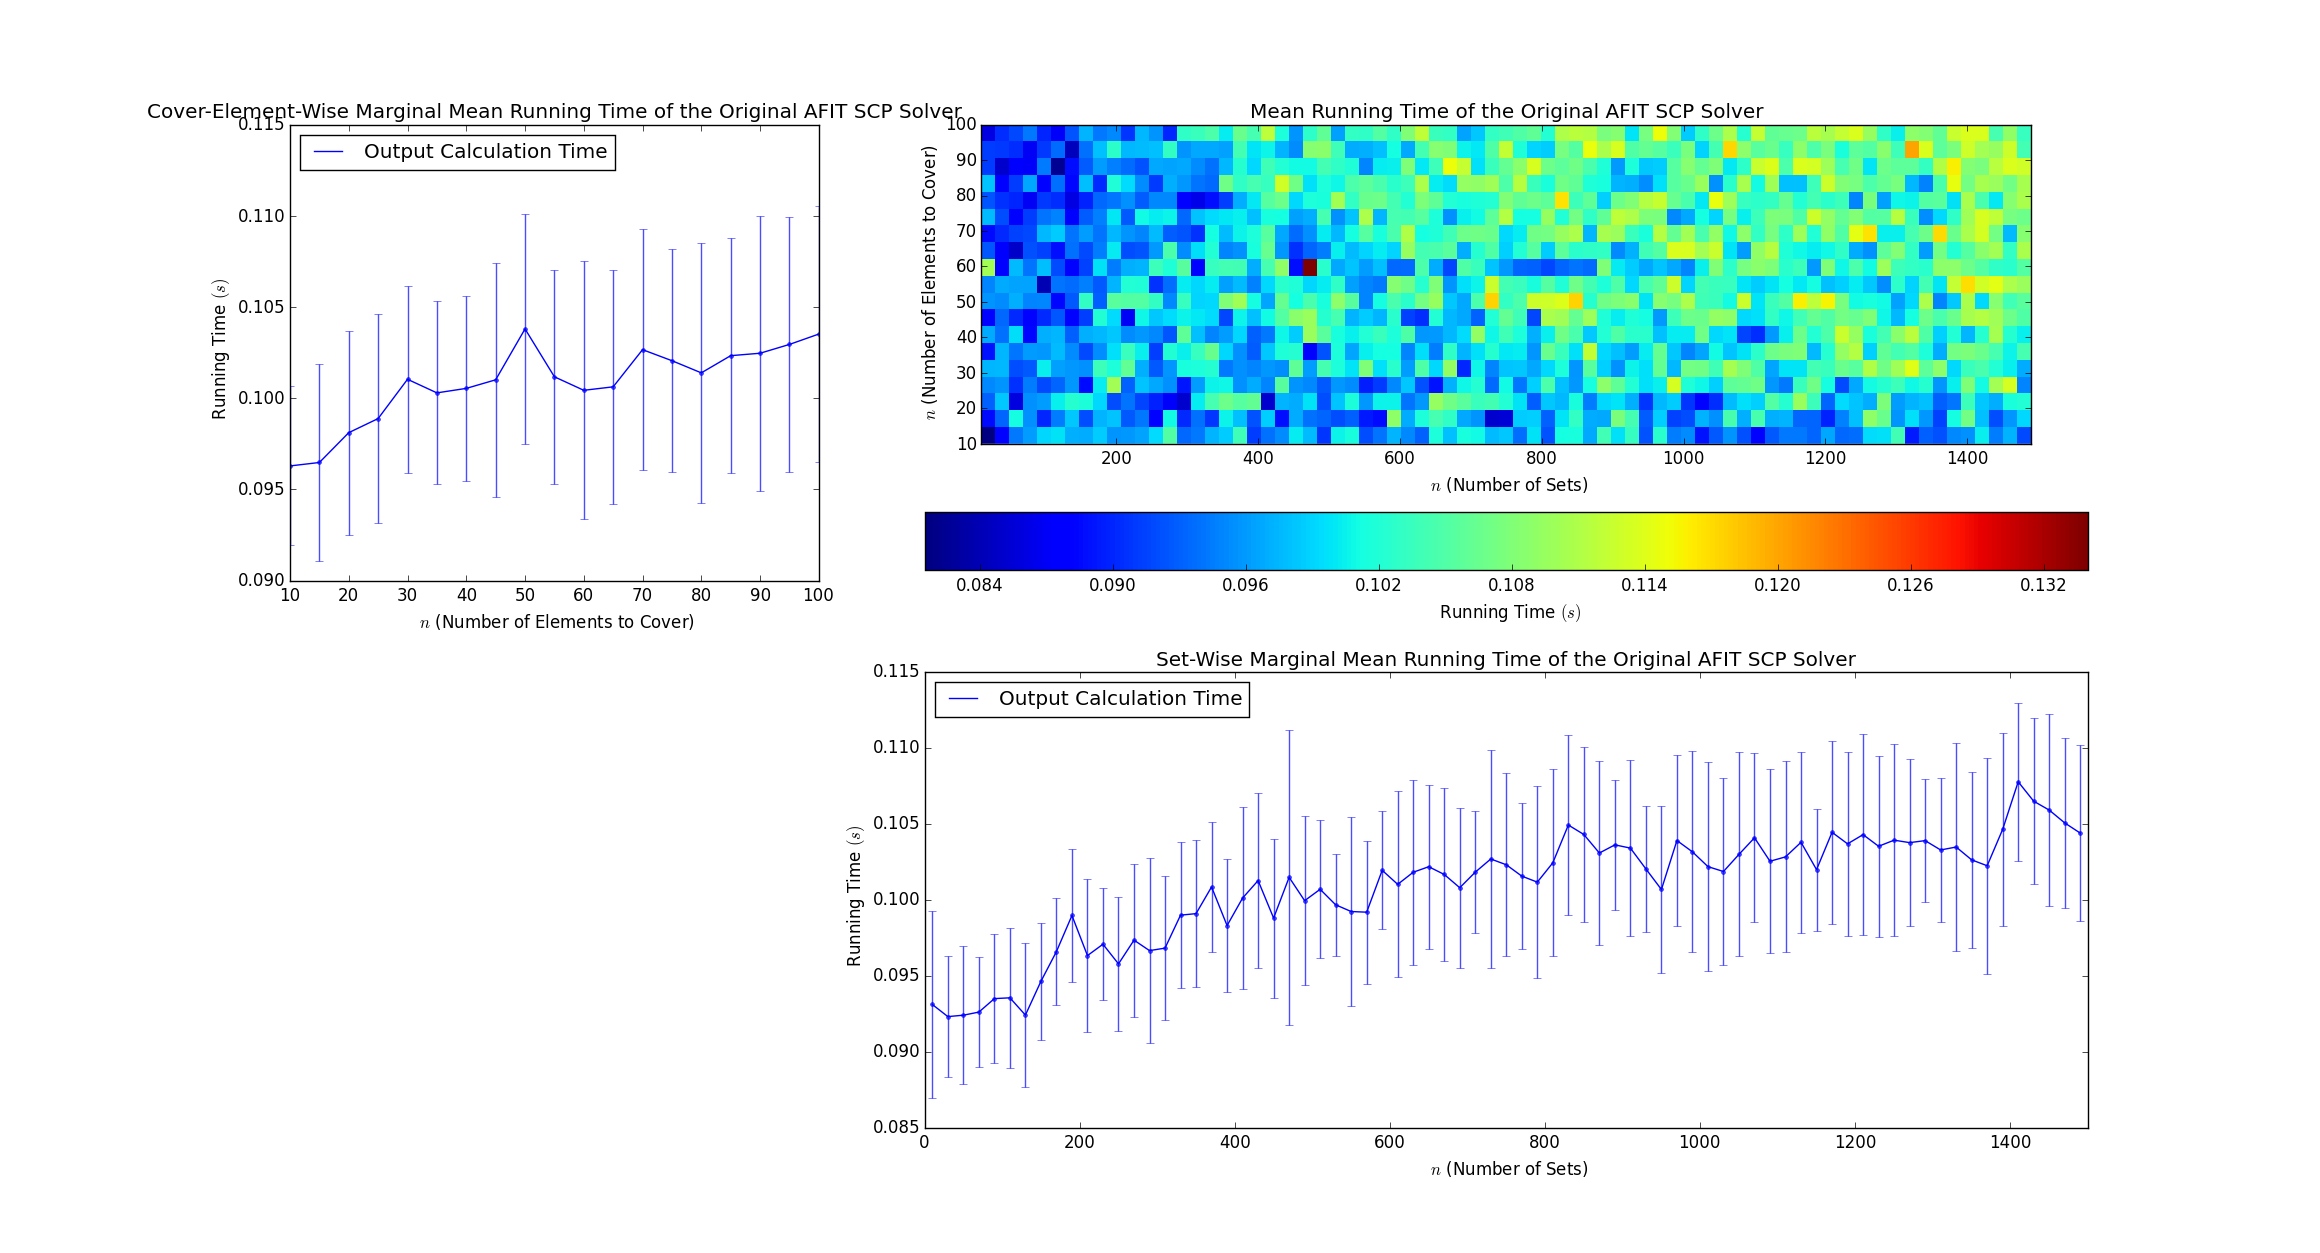
\includegraphics[width = 6.7in]{running_time_original_density0p3.png}}
	%  \vspace{2.0cm}
	\hfill
	
	%\vspace{-0.5cm}
	\caption{This figure displays the average running time performance of the original AFIT SCP Solver, over $20$ runs, for various instance configurations from the problem domain. All instances in this figure have a density of approximately $0.3$.}
	
\end{figure}

\begin{figure}[ht!]\label{fig:runtime_analysis_modified_density0p3}
	
	\centering
	\centerline{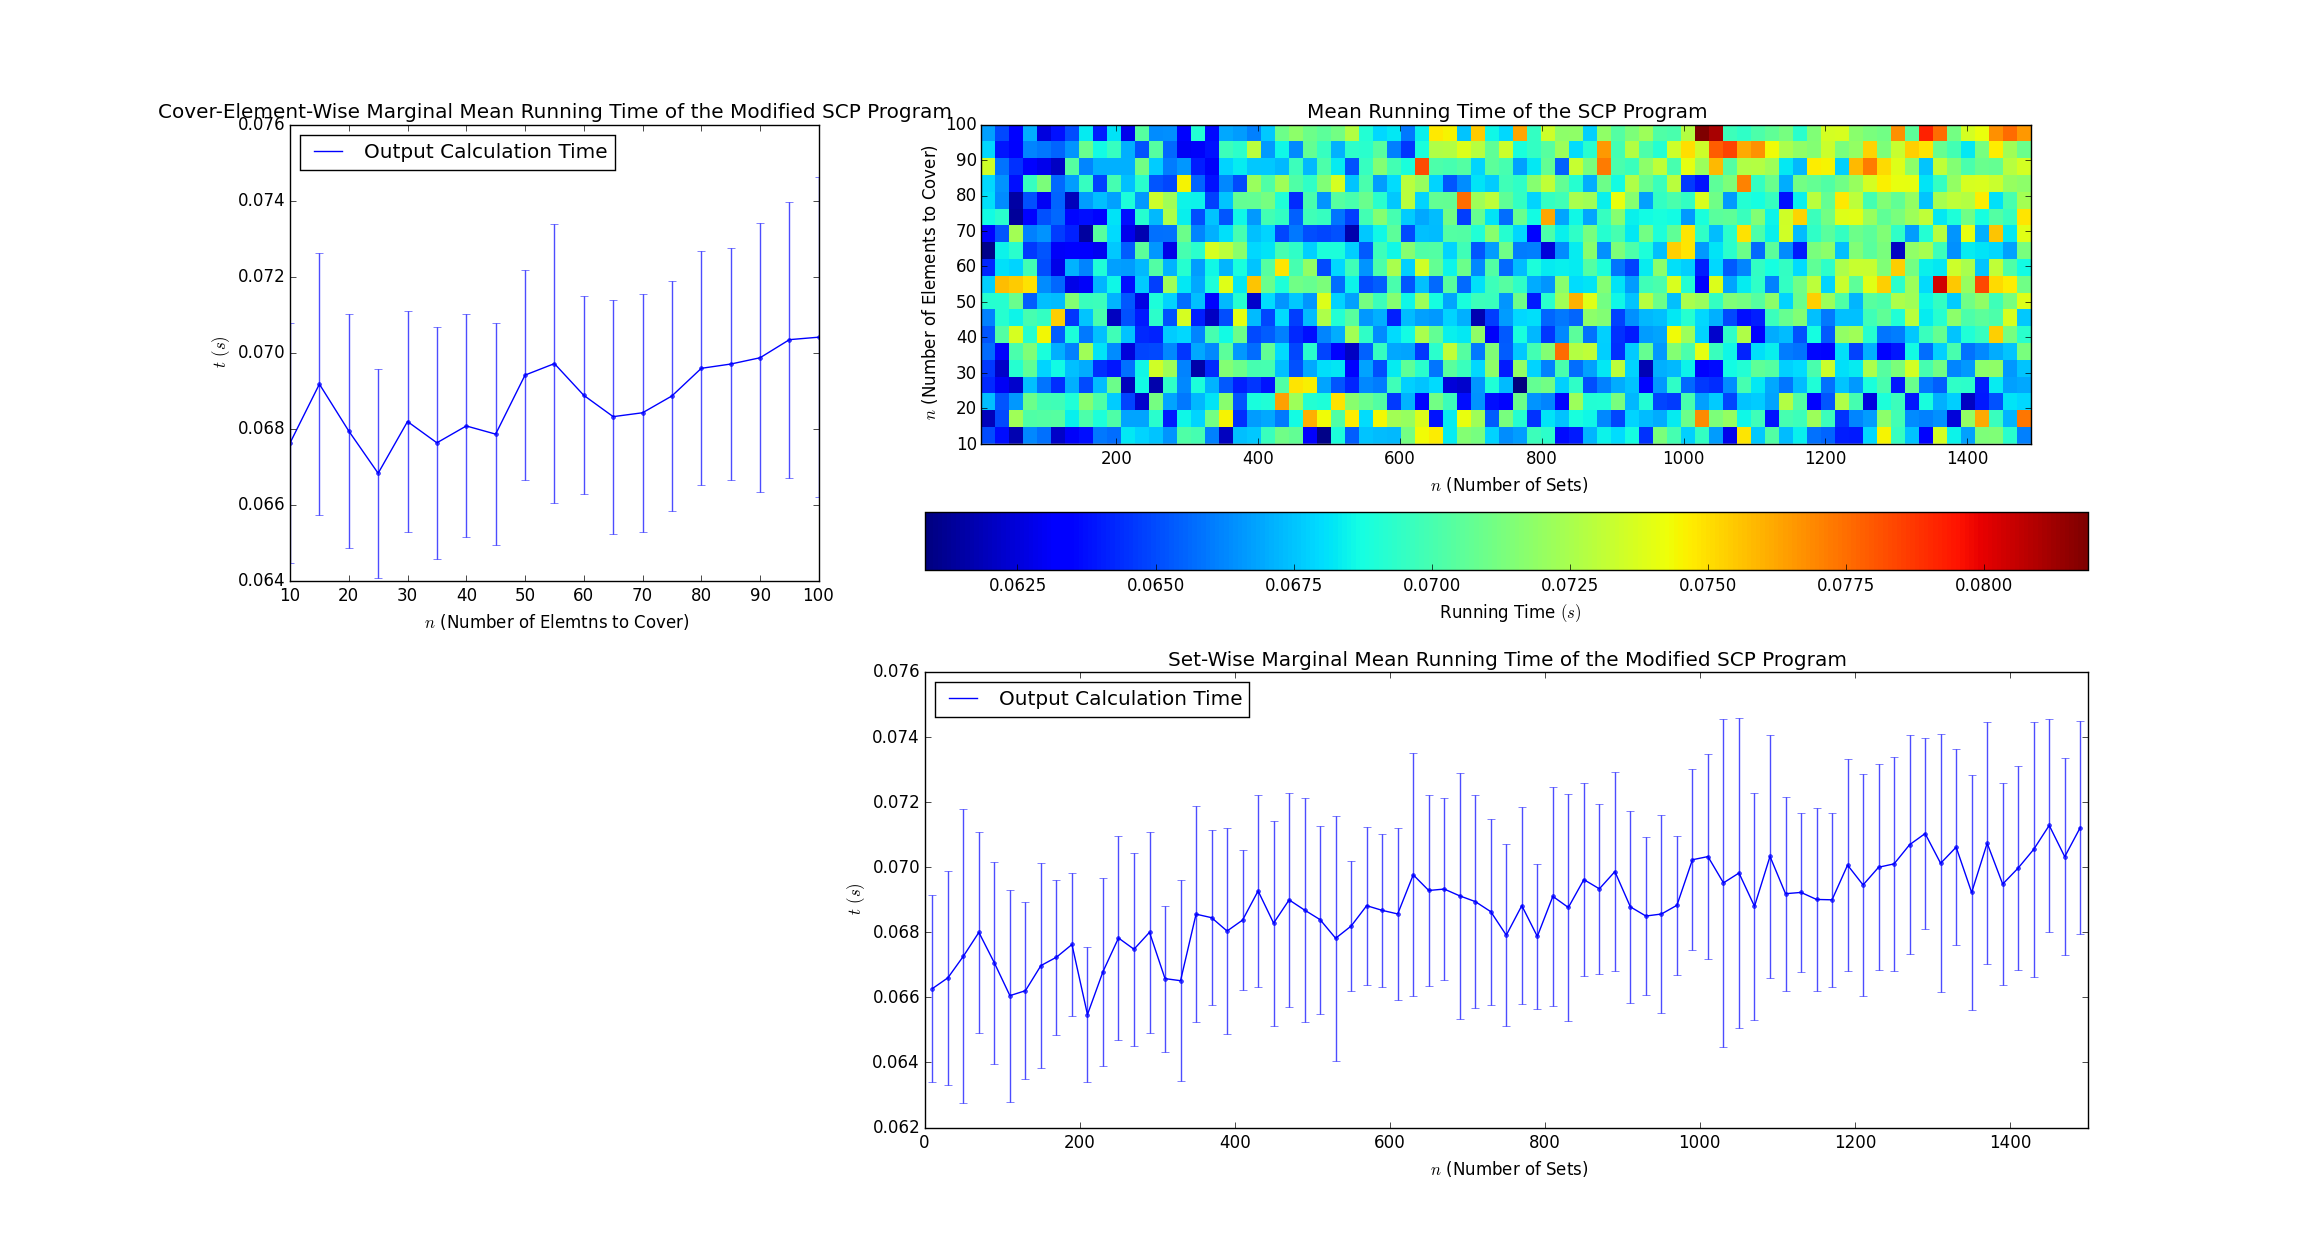
\includegraphics[width = 6.7in]{running_time_modified_density0p3_noout_noH1.png}}
	%  \vspace{2.0cm}
	\hfill
	
	%\vspace{-0.5cm}
	\caption{This figure displays the average running time performance of the modified AFIT SCP Solver, over $20$ runs, for various instance configurations from the problem domain. All instances in this figure have a density of approximately $0.3$.}
	
\end{figure}

\subsection{Search Tree [c.4]} 
[Jon?]
\section{AFIT SCP Program Software Engineering Practices} \label{scn:design}

[Jon] Does the AFIT SCP Solver employ good software engineering practices?

\section{AFIT SCP Program Complexity} \label{scn:design}

[Justin] Describe observed complexity.

\section{Integration} \label{scn:design}

[Jon] Discuss ease of understanding code in the AFIT SCP Solver. Discuss ease of standard interfaces.

\pagebreak
\appendix		% Appendix begins here

\section{Code Listing}

[Justin ] Talk about code briefly.
[Jon, you can add your source code below, once commented, then uncomment the \LaTeX -line. Neat, huh? Oh, and the caption needs to be a single sentence, otherwise it breaks. No idea why.]
%\lstinputlisting[language=Java, caption=Your caption here.]{yourSourceCode.java}

\bibliographystyle{IEEEtran}
\bibliography{algorthimBib}

\end{document}